\task{Имеется 8~внешне совершенно одинаковых свинцовых шариков, 
однако внутри одного из них сделана небольшая полость. Пользуясь 
только рычажными весами, определите, какой шарик с полостью. Весы 
можно использовать не более двух раз. Опишите свои действия и 
сделайте рисунок.}

\task{Вам даны кастрюля вместимостью 2~л, ведро с водой и чайник, в 
который необходимо как можно точнее отлить из ведра воду объемом 
1~л. Как это можно сделать?}

\task{Вам дана толстая общая тетрадь и линейка. Определите, как 
можно точнее, толщину тетрадного листа.}

\task{Расстояние от Ленинграда до Москвы 650~км, от Ленинграда до 
станции Бологое --- 280~км. Каково расстояние от Москвы до Бологого, 
если все три населенных пункта лежат на одной прямой?}

\task{Имеется 8~внешне совершенно одинаковых восковых шаров, однако 
внутрь одного из них закатана небольшая свинцовая дробинка. 
Пользуясь только рычажными весами, определите, в каком шаре 
находится дробинка. Весы можно использовать не более двух раз. 
Опишите свои действия и сделайте рисунок.}

\taskpic{Легкий воздушный шар и парусная яхта движутся прямолинейно 
равномерно параллельными курсами (в одном направлении). Яхта 
движется в 2~раза медленнее шара. Найдите физическую ошибку на 
рисунке. Сделайте верный рисунок и обоснуйте 
его.}{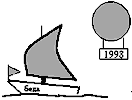
\includegraphics[width=3cm]{d07_06.png}}

\task{Имеются ведро сухого песка, ведро воды и мензурка. Предложите 
способ нахождения объема пустот в ведре сухого песка.}

\taskpic{На пляже имеются два магазина прохладительных напитков. 
Может ли отдыхающий идти так, чтобы к одному магазину он 
приближался, а расстояние до другого оставалось бы постоянным? 
Ответ обоснуйте и сопроводите рисунком. Первоначальное 
положение отдыхающего по отношению к магазинам приведено на 
рисунке (обозначено крестиком).}{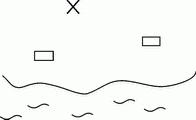
\includegraphics[width=4cm]{d07_08.png}}

\taskpic{Легкий воздушный шар и пароход движутся прямолинейно 
равномерно параллельными курсами (в одном направлении). Шар 
движется в 2~раза быстрее парохода. Найдите физическую ошибку на 
рисунке. Сделайте верный рисунок и обоснуйте 
его.}{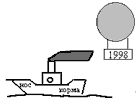
\includegraphics[width=3cm]{d07_09.png}}

\task{Три лучника стоят на одной линии на расстоянии 2~м друг от 
друга и стреляют последовательно через 1~с перпендикулярно линии 
стрельбы по длинной мишени, которая движется параллельно линии 
стрельбы со скоростью 0{,}5~м/с. На каком расстоянии друг от друга 
попадут стрелы в мишень, если известно, что все они летят с 
одинаковыми скоростями?}

\taskpic{В залив впадают два ручья. Можно ли на лодке двигаться по 
заливу так, чтобы, удаляясь от устья одного ручья, оставаться на 
постоянном расстоянии от устья другого? Ответ обоснуйте и 
сопроводите рисунком. Первоначальное расположение лодки по 
отношению к ручьям приведено на рисунке.}{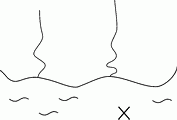
\includegraphics[width=4cm]{d07_11.png}}

\task{Плот плывет по течению реки в южном направлении. На плоту 
сидит мальчик и ловит рыбу. В какую сторону от положения 
вертикали будет отклоняться леска (и будет ли) находящаяся под 
водой?}

\task{В тире четыре стрелка, стоя на одной линии, стреляют в 
движущуюся мишень. На каком расстоянии будут следы от пуль на 
мишени, если она движется со скоростью 0{,}5~м/с параллельно линии 
стрельбы; стрелки стоят на расстоянии 1~м друг от друга и стреляют 
последовательно через 1~с?}

\task{Воздушный шар уносится ветром в северо-восточном 
направлении. В какую сторону будут развеваться флаги, украшающие 
шар?}

\task{Трем туристам необходимо за максимально короткий срок 
добраться из одного населенного пункта в другой. Как это сделать, 
если у них имеется лишь один одноместный велосипед? Скорость 
пешехода в 2 раза меньше велосипедиста. Построить график 
зависимость пройденного пути от времени для всех тел, 
участвующих в движении.}

\task{У Вас есть моток тонкой проволоки, карандаш и тетрадь в 
клетку. Как можно определить диаметр поперечного сечения 
проволоки?}

\task{Имеются ведро сухого песка, ведро воды и мензурка. Предложите 
способ нахождения объема пустот в ведре сухого песка.}

\task{За сутки молодой бамбук может вырасти на 86,4 см. На сколько он 
вырастает за секунду?}

\task{На какой угол поворачивается Земля вокруг своей оси за 1~мин?}

\task{Сколько потребовалось бы времени для того, чтобы уложить в 
ряд кубики, объемом 1~мм$^3$ каждый, взятые в таком количестве, 
сколько содержится их в 1~м$^3$ , если на укладку одного кубика 
затрачивается время, равное 1~с?}

\task{Четыре мальчика отправились из одного населенного пункта в 
другой, имея лишь один одноместный велосипед. Известно, что 
скорость велосипедиста в 4~раза больше скорости пешехода. Что 
необходимо сделать, чтобы как можно быстрее проделать этот путь? 
Построить график зависимости пройденного пути от времени для 
всех тел, участвующих в движении.}

\task{Мальчик идет из дома в школу, расстояние от дома до которой 
1200~м. Он всегда приходил в школу в одно и то же время. Но на трети 
пути он вспоминает, что забыл дневник, и решает вернуться домой 
за дневником. С какой скоростью он должен бежать с этого момента , 
чтобы успеть в школу в то же время, если обычно он идет с 
постоянной скоростью 7{,}2~км/ч?}

\task{Имеются ведро сухого песка, ведро воды и мензурка. Предложите 
способ нахождения собственного объема песчинок в ведре сухого 
песка.}

\taskpic{Во время археологических раскопок была найдена старинная 
бутылка, нижняя часть которой имеет форму параллелепипеда и по 
объему составляет около $\frac{2}{3}$ от всей бутылки. Верхняя часть 
бутылки имеет неправильную форму. Имея в распоряжении линейку, 
пробку к этой бутылке и неограниченные запасы воды, определите 
объем этой бутылки.}{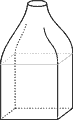
\includegraphics[width=1.5cm]{d07_24.png}}

\task{Почему при резком торможении передним колесом велосипеда 
есть опасность перелететь через руль?}

\taskpic{Вода вытекает с постоянной скоростью $v$ из двух одинаковых 
труб в одну трубу с площадью поперечного сечения в 3~раза большей, 
чем у каждой из двух предыдущих труб. Какова скорость $u$ течения 
воды в трубе большого сечения? Вода полностью заполняет 
трубы.}{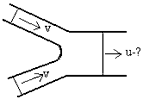
\includegraphics[width=3cm]{d07_26.png}}

\task{Имеются рычажные весы с чашами различной массы, набор 
одинаковых кубиков, набор одинаковых шариков. Весы находятся в 
равновесии, если положить: на левую чашу 2~кубика, на правую 
3~шарика; или на левую чашу 1~шарик, на правую 1~кубик. Какая чаша 
весов опустится, если положить: на левую чашу 1~кубик, на правую 
1~шарик? Ответ обоснуйте.}

\task{На одной из линий метрополитена все станции расположены на 
одинаковом расстоянии. На преодоление этого расстояния поезд 
метро тратит 4~минуты. В каждую сторону поезда ходят один раз в 
3~минуты. На одной из станций машинист заметил, что на 
противоположной платформе стоит поезд. Через какое время он 
снова увидит поезд, следующий в противоположную сторону?}

\task{На линии метро расположено 10~станций на одинаковом 
расстоянии друг от друга. Между соседними станциями поезд 
движется 3~минуты. Линию обслуживают 18~поездов. К очередному 
празднику было решено ввести новую конечную станцию. Её 
расположили так, что время движения от неё до ближайшей станции 
метро составило 6~минут. На всех станциях поезд проводит 3~минуты. 
На конечных станциях поезд также стоит 3~минуты, после чего едет в 
обратном направлении. Сколько нужно ввести дополнительных 
поездов, чтобы интервал между их появлениями (в одном 
направлении) на станциях остался прежним?}

\task{С территории военной части Х, расположенной вблизи города Y, 
одновременно выехали три танка. Ехали они по одной дороге, и 
скорость каждого из них была постоянна. Скорость первого танка 
равнялась $v_1 = 30\mbox{ км/ч}$, скорость второго $v_2 = 20\mbox{ км/ч}$. Первый 
танк въехал в город Y в 19{.}00, второй танк --- в 20{.}00, а третий танк --- в 
21{.}00. Найдите скорость третьего танка.}
